%
% This is a borrowed LaTeX template file for lecture notes for CS267,
% Applications of Parallel Computing, UCBerkeley EECS Department.
% Now being used for CMU's 10725 Fall 2012 Optimization course
% taught by Geoff Gordon and Ryan Tibshirani.  When preparing
% LaTeX notes for this class, please use this template.
%
% To familiarize yourself with this template, the body contains
% some examples of its use.  Look them over.  Then you can
% run LaTeX on this file.  After you have LaTeXed this file then
% you can look over the result either by printing it out with
% dvips or using xdvi. "pdflatex template.tex" should also work.
%

\documentclass[twoside]{article}
\setlength{\oddsidemargin}{0.25 in}
\setlength{\evensidemargin}{-0.25 in}
\setlength{\topmargin}{-0.6 in}
\setlength{\textwidth}{6.5 in}
\setlength{\textheight}{8.5 in}
\setlength{\headsep}{0.75 in}
\setlength{\parindent}{0 in}
\setlength{\parskip}{0.1 in}

%
% ADD PACKAGES here:
%

\usepackage{amsmath,amsfonts,graphicx}
\graphicspath{ {./images/} }

%
% The following commands set up the lecnum (lecture number)
% counter and make various numbering schemes work relative
% to the lecture number.
%
\newcounter{lecnum}
\renewcommand{\thepage}{\thelecnum-\arabic{page}}
\renewcommand{\thesection}{\thelecnum.\arabic{section}}
\renewcommand{\theequation}{\thelecnum.\arabic{equation}}
\renewcommand{\thefigure}{\thelecnum.\arabic{figure}}
\renewcommand{\thetable}{\thelecnum.\arabic{table}}

%
% The following macro is used to generate the header.
%
\newcommand{\lecture}[4]{
    \pagestyle{myheadings}
    \thispagestyle{plain}
    \newpage
    \setcounter{lecnum}{#1}
    \setcounter{page}{1}
    \noindent
    \begin{center}
    \framebox{
        \vbox{\vspace{2mm}
    \hbox to 6.28in { {\bf CPSC 421: Introduction to Theory of Computing
    \hfill Winter Term 1 2018-19} }
        \vspace{4mm}
        \hbox to 6.28in { {\Large \hfill Lecture #1: #2  \hfill} }
        \vspace{2mm}
        \hbox to 6.28in { {\it Lecturer: #3 \hfill Scribes: #4} }
        \vspace{2mm}}
    }
    \end{center}
    \markboth{Lecture #1: #2}{Lecture #1: #2}

%    {\bf Note}: {\it LaTeX template courtesy of UC Berkeley EECS dept.}
%
%    {\bf Disclaimer}: {\it These notes have not been subjected to the
%    usual scrutiny reserved for formal publications.  They may be distributed
%    outside this class only with the permission of the Instructor.}
%    \vspace*{4mm}
}
%
% Convention for citations is authors' initials followed by the year.
% For example, to cite a paper by Leighton and Maggs you would type
% \cite{LM89}, and to cite a paper by Strassen you would type \cite{S69}.
% (To avoid bibliography problems, for now we redefine the \cite command.)
% Also commands that create a suitable format for the reference list.
\renewcommand{\cite}[1]{[#1]}
\def\beginrefs{\begin{list}%
        {[\arabic{equation}]}{\usecounter{equation}
            \setlength{\leftmargin}{2.0truecm}\setlength{\labelsep}{0.4truecm}%
            \setlength{\labelwidth}{1.6truecm}}}
\def\endrefs{\end{list}}
\def\bibentry#1{\item[\hbox{[#1]}]}

%Use this command for a figure; it puts a figure in wherever you want it.
%usage: \fig{NUMBER}{SPACE-IN-INCHES}{CAPTION}
\newcommand{\fig}[3]{
            \vspace{#2}
            \begin{center}
            Figure \thelecnum.#1:~#3
            \end{center}
    }
% Use these for theorems, lemmas, proofs, etc.
\newtheorem{theorem}{Theorem}[lecnum]
\newtheorem{lemma}[theorem]{Lemma}
\newtheorem{proposition}[theorem]{Proposition}
\newtheorem{claim}[theorem]{Claim}
\newtheorem{corollary}[theorem]{Corollary}
\newtheorem{definition}[theorem]{Definition}
\newenvironment{proof}{{\bf Proof:}}{\hfill\rule{2mm}{2mm}}

% **** IF YOU WANT TO DEFINE ADDITIONAL MACROS FOR YOURSELF, PUT THEM HERE:

\newcommand\E{\mathbb{E}}

\begin{document}
%FILL IN THE RIGHT INFO.
%\lecture{**LECTURE-NUMBER**}{**DATE**}{**LECTURER**}{**SCRIBE**}
\lecture{5}{September 14}{Nicholas Harvey}{Kaitian Xie}
%\footnotetext{These notes are partially based on those of Nigel Mansell.}

\section{Regular Expressions}
We will ``show'': A language is a regular iff it can be described by a \underline{regular expression}.

$R$:
\begin{itemize}
  \item $0^*1^*$
  \item $\Sigma^*001\Sigma^*$
  \item $(\Sigma\Sigma)^*$
  \item $\Sigma^*1\Sigma^*1\Sigma^*$
\end{itemize}

\underline{Shorthand}: $\Sigma = (a_1|a_2|\cdots|a_k) \text{ where } \Sigma  = a_1a_2\cdots a_k$

$L(R)$: the set of strings generated by regular expression $R$.
\begin{itemize}
  \item $\{0^i1^j: i, j \geq 0\}$
  \item \{all strings containing $001$ as a substring\}
  \item \{all strings of even length\}
  \item $\{w: w \text{ contains at least three 1s}\}$
\end{itemize}

$\Leftarrow$: Any regular expression can be converted into an equivalent NFA.

$\Rightarrow$: Idea: generalize NFAs by allowing arbitrary R.Es as labels on their transitions. Keep simplifying.

\underline{Limits to the power of Finite Automata}

Can any language be described by a F.A?

\underline{Example 1}: Suppose $L$ is a finite language (i.e. $L$ is finite). Is $L$ regular? Yes

Why? Suppose $L = \{x_1, \cdots, x_n\}.$

We can define $L_i = \{x_i\}$. This is regular. We know $L_1 \cup L_2 $ is regular, so $L_1 \cup L_2 \cup \cdots \cup L_n$ is regular.
 
This fails if $L$ is infinite because we could get an ``Infinite Automaton''.

\underline{Example 2}: Suppose $L$ is regular. Define $L^2 = \{xy: x \in L \text{ and } y \in L\}$

This is regular: it is $L \circ L$.

\underline{Example 3}: $L^{dup} = \{xx: x \in L\}$

Is this regular? It depends $\cdots$

If $L$ is finite, $L^{dup}$ is finite, hence regular.

If $L = L(1^*)$, then $L^{dup} = \{1^{2i}: i \geq 0\} = L((11)^*)$

If $L = \Sigma^*$, $L^{dup} = \{xx: x \in \Sigma^*\}$. Is this regular?

\underline{Intuitive argument}: $\{xx: x \in \Sigma^*\}$ is not regular.

\begin{itemize}
  \item With a F.A. its states are its ``memory''.
  \item Any F.A. accepting $L^{dup}$ ``must remember'' the first half to compare to the second half.
  \item So F.A. must remember arbitrary large information, but it can't.
\end{itemize}

\underline{Idea about finite automaton}:

\begin{figure*}[ht]
  \centering
  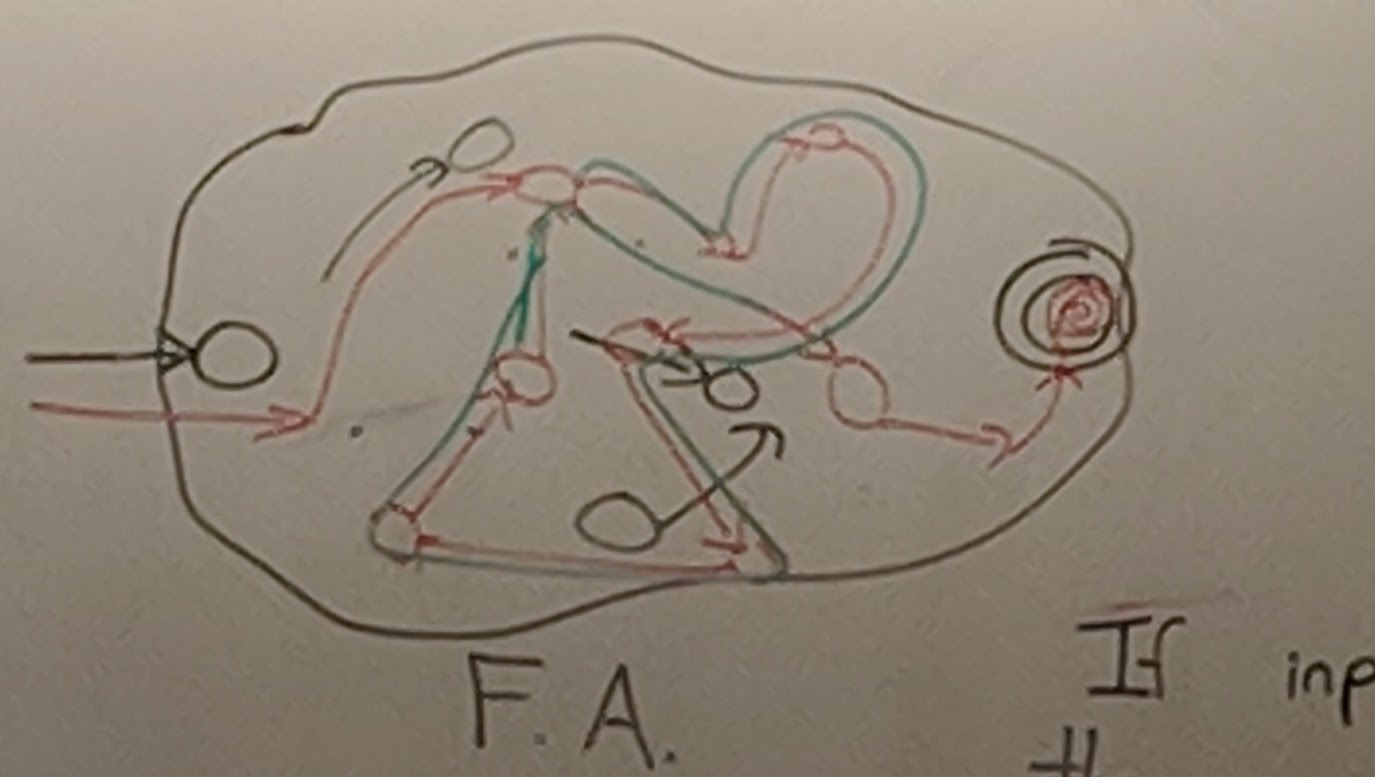
\includegraphics[scale=0.3]{img1}
\end{figure*}

\begin{itemize}
  \item $\rightarrow$ ``computation path'', transitions followed when processing input
\end{itemize}

If input is very long, this computation path must have a \underline{cycle}.

\end{document}
